\documentclass{article}

\usepackage[final]{nips_2017}

\usepackage[utf8]{inputenc} % allow utf-8 input
\usepackage[T1]{fontenc}    % use 8-bit T1 fonts
\usepackage{hyperref}       % hyperlinks
\usepackage{url}            % simple URL typesetting
\usepackage{booktabs}       % professional-quality tables
\usepackage{amsfonts}       % blackboard math symbols
\usepackage{nicefrac}       % compact symbols for 1/2, etc.
\usepackage{microtype}      % microtypography
\usepackage{graphicx}

\title{Pun Classification and Location}

% The \author macro works with any number of authors. There are two
% commands used to separate the names and addresses of multiple
% authors: \And and \AND.
%
% Using \And between authors leaves it to LaTeX to determine where to
% break the lines. Using \AND forces a line break at that point. So,
% if LaTeX puts 3 of 4 authors names on the first line, and the last
% on the second line, try using \AND instead of \And before the third
% author name.

\author{
	Shantanu Karnwal
	\texttt{shantanu.karnwal@colorado.edu} \\
	\And
	Amir Kashipazha
	\texttt{amirhossein.kashipazha@colorado.edu} \\
	\And
	Brandon Boylan-Peck
	\texttt{brbo9266@colorado.edu} \\
	\And
	Cathlyn Stone\\
	\texttt{cathlyn.stone@colorado.edu} \\
	\And
	Kenneth Hunter Wapman\\
	\texttt{kennethwapman@colorado.edu} \\
}

\begin{document}

\maketitle

\begin{abstract}
	Pun identification and location are challenging natural language processing 
	tasks. We implemented several algorithms for both, with results which 
	were comparable to those outlined in the SemEval conference which originally
	defined the tasks.
\end{abstract}

%%%%%%%%%%%%%%%%%%%%%%%%%%%%%%%%%%%%%%%%%%%%%%%%%%%%%%%%%%%%%%%%%%%%%%%%%%%%%%%
% Problem Description
%%%%%%%%%%%%%%%%%%%%%%%%%%%%%%%%%%%%%%%%%%%%%%%%%%%%%%%%%%%%%%%%%%%%%%%%%%%%%%%

\section{Overview}

\subsection{Pun Structure}

here we will talk about what puns are
\begin{itemize}

\item homographic
\item heterographic
\item other types

\end{itemize}

here we will talk about the problems we worked on.

\begin{center}
	homographic pun example
  % \url{https://cmt.research.microsoft.com/NIPS2017/}
\end{center}

\begin{center}
	heterographic pun example
  % \url{https://cmt.research.microsoft.com/NIPS2017/}
\end{center}

Please read carefully the instructions below and follow them
faithfully.

\subsection{Motivation}


\subsection{Tasks}

section references \ref{pun_detection}, \ref{pun_location}, and
\ref{conclusion} below.

%%%%%%%%%%%%%%%%%%%%%%%%%%%%%%%%%%%%%%%%%%%%%%%%%%%%%%%%%%%%%%%%%%%%%%%%%%%%%%%
% Pun Detection
%%%%%%%%%%%%%%%%%%%%%%%%%%%%%%%%%%%%%%%%%%%%%%%%%%%%%%%%%%%%%%%%%%%%%%%%%%%%%%%

\section{Pun Detection}
\label{pun_detection}

here we will talk about pun detection and our algorithms.

\subsection{Baseline}

\subsection{Algorithms}

\subsection{Feature Comparison}

%%%%%%%%%%%%%%%%%%%%%%%%%%%%%%%%%%%%%%%%%%%%%%%%%%%%%%%%%%%%%%%%%%%%%%%%%%%%%%%
% Pun Location
%%%%%%%%%%%%%%%%%%%%%%%%%%%%%%%%%%%%%%%%%%%%%%%%%%%%%%%%%%%%%%%%%%%%%%%%%%%%%%%
\section{Pun Location}
\label{pun_location}

\subsection{Baseline}

\subsection{Algorithms}

\subsection{Feature Comparison}
We introduced various features to improve accuracy Table \ref{tab:List_of_features}. Indexes in this table represent the index of each feature in the code and figures we made for feature analysis. Features were added to the code one by one to find whether they improve accuracy. In general, we saw accuracy improved with adding features. Accuracy change behave differently against each feature.\\
Next step was to find what feature combination led to the largest accuracy. We designed a code to find various combinations of features. The code generated list of indexes of all possible number of feature a code can have. Length of the list was between one to number of feature, 1 to 16. With 16 feature we could have 65535 possible combination. The pun detection code took about 60s to be done. If we wanted to test all these combination it took about 1092 hours. In this regards, we did trail and error run to see what feature improve accuracy. Finally, we used 11 features that indexed from 0 to 10 in the table \ref{tab:List_of_features} for feature comparison. \\
With using 11 feature we were able to create 2047 features combination. Then we calculated accuracy for detection of homographic and heterographic puns. This let to 4089 runs. We found 100 percent accuracy anytime unigaram appears in any combination which is sign on over fitting. So we eliminated this feature form analysis. \\
Figures \ref{fig:ACC_Train_Homo} and \ref{fig:ACC_Train_Hetero} shows the 10 largest accuracy of feature combination for training set of homographic and heterographic pun. These figure shows accuracy of training set of pun reached more than 96 percent for both pun. Figures \ref{fig:ACC_Test_Homo} and \ref{fig:ACC_Test_Hetero} shows the 10 largest accuracy of testing set for homographic and heterographic. These figures shows accuracy of testing sets of pun reached above 83 percent.\\




\begin {table}
\caption {List of Features and Their Indexes in Code} 
\label{tab:List_of_features} 
\begin{center}
\begin{tabular}{ l|l } 
\hline
\textbf{Index} 	&	\textbf{Feaute Name}	\\
\hline
0	&	Lesk Algorithm	\\
1	&	Pos	\\
2	&	tfidf	\\
3	&	Embeddings	\\
4	&	Unigram	\\
5	&	Number of Homophone in Pun	\\
6	&	Number of Each Homophone in Pun	\\
7	&	Homophone is in Pun or Not	\\
8	&	Idiom is in Pun or Not	\\
9	&	Antonyms is in Pun or Not	\\
10	&	Homonym is in Pun or Not	\\
11	&	Bigram	\\
12	&	Trigram	\\
13	&	Positives	\\
14	&	Negatives	\\
15	&	All or First Caps	\\
\hline
  
\end{tabular}
\end{center}
\end{table}


\begin{figure}
  \centering
  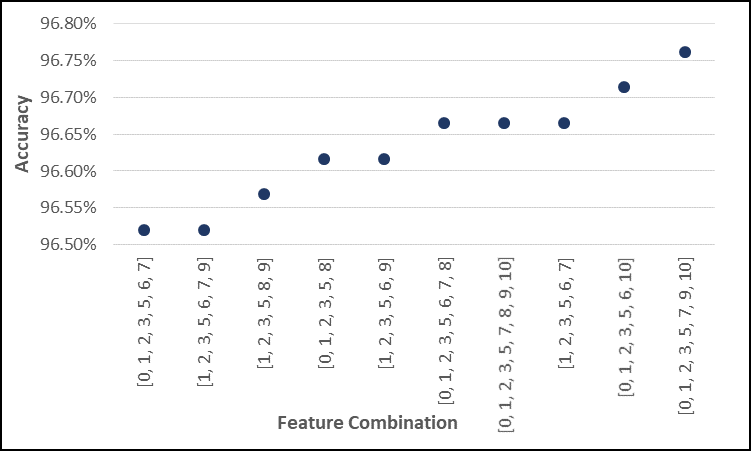
\includegraphics[width=15cm]{figures/Accuracy_on_Training_Set_for_Homographic_Pun.png}
  \caption{Accuracy on Training Set for Homographic Pun}
  \label{fig:ACC_Train_Homo} 
\end{figure}

\begin{figure}
  \centering
  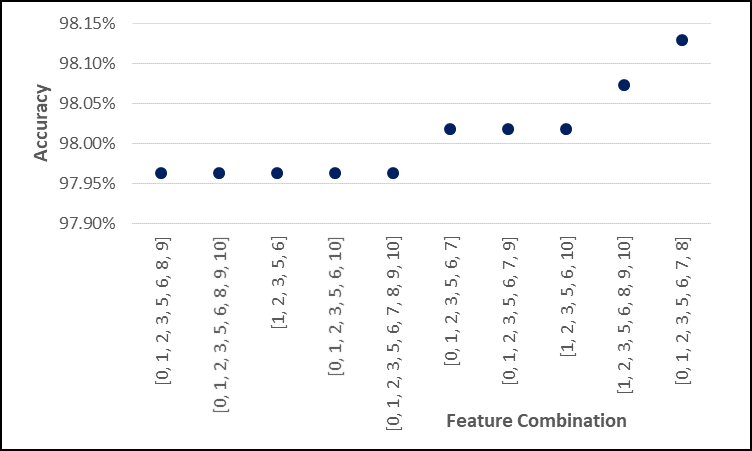
\includegraphics[width=15cm]{figures/Accuracy_on_Training_Set_for_Heterographic_Pun.png}
  \caption{Accuracy on Training Set for Heterographic Pun}
  \label{fig:ACC_Train_Hetero}
\end{figure}



\begin{figure}
  \centering
  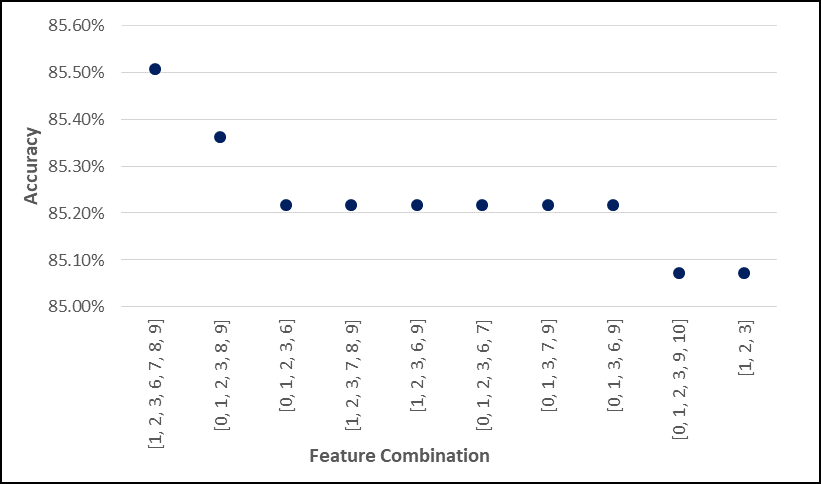
\includegraphics[width=15cm]{figures/Accuracy_on_Test_Set_for_Homographic_Pun.png}
  \caption{Accuracy on Testing Set for Homographic Pun}
  \label{fig:ACC_Test_Homo}
\end{figure}


\begin{figure}
  \centering
  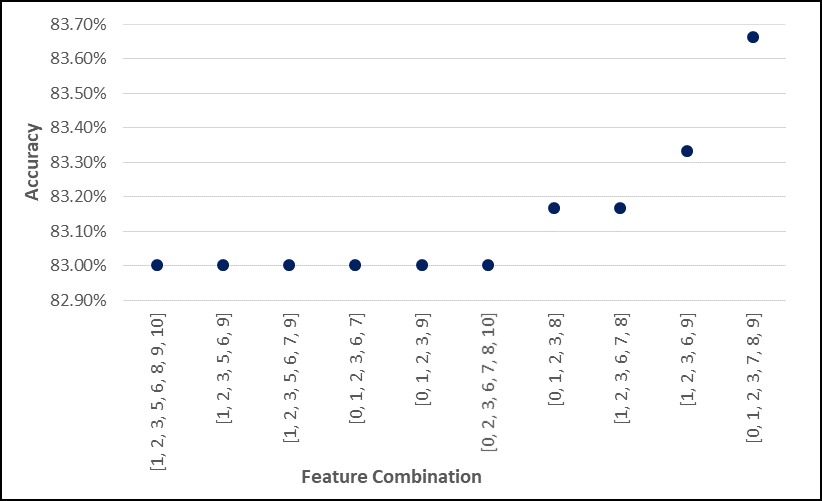
\includegraphics[width=15cm]{figures/Accuracy_on_Test_Set_for_Heterographic_Pun.png}
  \caption{Accuracy on Testing Set for Heterographic Pun}
  \label{fig:ACC_Test_Hetero}
\end{figure}




\section{Results}
\label{results}

\subsection{Pun Detection}
Here's how we think we did.
\subsubsection{Evaluation}
\subsubsection{Results}
here are our results. here's the baseline. here's semeval's

\subsubsection{Error Analysis}

\subsection{Pun Location}
Here's how we think we did.
\subsubsection{Evaluation}
f score etc etc
\subsubsection{Results}
here are our results. here's the baseline. here's semeval's
\subsubsection{Error Analysis}

%%%%%%%%%%%%%%%%%%%%%%%%%%%%%%%%%%%%%%%%%%%%%%%%%%%%%%%%%%%%%%%%%%%%%%%%%%%%%%%
% Conclusion
%%%%%%%%%%%%%%%%%%%%%%%%%%%%%%%%%%%%%%%%%%%%%%%%%%%%%%%%%%%%%%%%%%%%%%%%%%%%%%%

\section{Conclusion}
\label{conclusion}

\subsection{who did what}
\subsection{what went well}
\subsection{what we could have done better}

\subsubsection*{Acknowledgments}

here's where we acknowledge stuff

%%%%%%%%%%%%%%%%%%%%%%%%%%%%%%%%%%%%%%%%%%%%%%%%%%%%%%%%%%%%%%%%%%%%%%%%%%%%%%%
% References
%%%%%%%%%%%%%%%%%%%%%%%%%%%%%%%%%%%%%%%%%%%%%%%%%%%%%%%%%%%%%%%%%%%%%%%%%%%%%%%
\section*{References}

\medskip

\small

[1] Alexander, J.A.\ \& Mozer, M.C.\ (1995) Template-based algorithms
for connectionist rule extraction. In G.\ Tesauro, D.S.\ Touretzky and
T.K.\ Leen (eds.), {\it Advances in Neural Information Processing
  Systems 7}, pp.\ 609--616. Cambridge, MA: MIT Press.

[2] Bower, J.M.\ \& Beeman, D.\ (1995) {\it The Book of GENESIS:
  Exploring Realistic Neural Models with the GEneral NEural SImulation
  System.}  New York: TELOS/Springer--Verlag.

[3] Hasselmo, M.E., Schnell, E.\ \& Barkai, E.\ (1995) Dynamics of
learning and recall at excitatory recurrent synapses and cholinergic
modulation in rat hippocampal region CA3. {\it Journal of
  Neuroscience} {\bf 15}(7):5249-5262.

%%%%%%%%%%%%%%%%%%%%%%%%%%%%%%%%%%%%%%%%%%%%%%%%%%%%%%%%%%%%%%%%%%%%%%%%%%%%%%%
% Misc Style examples
%%%%%%%%%%%%%%%%%%%%%%%%%%%%%%%%%%%%%%%%%%%%%%%%%%%%%%%%%%%%%%%%%%%%%%%%%%%%%%%
\section{Style Stuff}
\verb+this is code-ish looking+ 

here's a percent: $\sim$$15\%$
\textbf{boldboldbold}
\emph{italics}

here's a fraction: \nicefrac{1}{4}

\paragraph{}This is paragraphed
\begin{verbatim}
   \citet{hasselmo} investigated\dots
\end{verbatim}
produces
\begin{quote}
  Hasselmo, et al.\ (1995) investigated\dots
\end{quote}

ref number:\ [4]

footnotes.\footnote{they go after the period}

\begin{figure}[h]
  \centering
  \fbox{\rule[-.5cm]{0cm}{4cm} \rule[-.5cm]{4cm}{0cm}}
  \caption{Sample figure caption.}
\end{figure}

Table~\ref{sample-table}.

use \verb+booktabs+ package for tables
\begin{center}
  \url{https://www.ctan.org/pkg/booktabs}
\end{center}

\begin{table}[t]
  \caption{Sample table title}
  \label{sample-table}
  \centering
  \begin{tabular}{lll}
    \toprule
    \multicolumn{2}{c}{Part}                   \\
    \cmidrule{1-2}
    Name     & Description     & Size ($\mu$m) \\
    \midrule
    Dendrite & Input terminal  & $\sim$100     \\
    Axon     & Output terminal & $\sim$10      \\
    Soma     & Cell body       & up to $10^6$  \\
    \bottomrule
  \end{tabular}
\end{table}

\end{document}
